%% PARTE 3: EJERCICIOS PROPUESTOS
%% Geometría Analítica - Circunferencia - Grado 10
%% Este archivo contiene ejercicios propuestos con soluciones completas

\section{Ejercicios Propuestos}

% NIVEL BÁSICO - Ejercicios 1-3

\begin{ejercicio}[title={Ejercicio 1: Ecuación canónica - Nivel BÁSICO}}]
Dados los siguientes centros y radios, hallar la ecuación canónica de la circunferencia:
\begin{enumerate}[a)]
    \item Centro $(2,3)$, radio $r=5$
    \item Centro $(-1,4)$, radio $r=3$
    \item Centro $(0,-2)$, radio $r=6$
\end{enumerate}
\end{ejercicio}

\begin{ejercicio}[title={Ejercicio 2: Hallar centro y radio - Nivel BÁSICO}}]
Determinar el centro y el radio de las siguientes circunferencias dadas en forma canónica:
\begin{enumerate}[a)]
    \item $(x-4)^2 + (y+1)^2 = 16$
    \item $(x+3)^2 + (y-2)^2 = 49$
    \item $x^2 + (y-5)^2 = 36$
\end{enumerate}
\end{ejercicio}

\begin{ejercicio}[title={Ejercicio 3: Convertir ecuación general a canónica - Nivel BÁSICO}}]
Convertir las siguientes ecuaciones de forma general a forma canónica e identificar centro y radio:
\begin{enumerate}[a)]
    \item $x^2 + y^2 - 6x + 4y - 12 = 0$
    \item $x^2 + y^2 + 8x - 2y + 1 = 0$
    \item $x^2 + y^2 - 10y + 9 = 0$
\end{enumerate}
\end{ejercicio}

% NIVEL INTERMEDIO - Ejercicios 4-7

\begin{ejercicio}[title={Ejercicio 4: Ecuación dado centro y punto - Nivel INTERMEDIO}}]
Hallar la ecuación canónica de la circunferencia con centro en $C$ y que pasa por el punto $P$:
\begin{enumerate}[a)]
    \item Centro $C(1,2)$, punto $P(4,6)$
    \item Centro $C(-2,3)$, punto $P(1,7)$
    \item Centro $C(0,0)$, punto $P(3,-4)$
\end{enumerate}
\end{ejercicio}

\begin{ejercicio}[title={Ejercicio 5: Posición de puntos - Nivel INTERMEDIO}}]
Determinar si los siguientes puntos están dentro, sobre o fuera de la circunferencia $(x-2)^2 + (y+1)^2 = 25$:
\begin{enumerate}[a)]
    \item Punto $A(5,3)$
    \item Punto $B(2,4)$
    \item Punto $C(-1,-3)$
\end{enumerate}
\end{ejercicio}

\begin{ejercicio}[title={Ejercicio 6: Intersección recta-circunferencia - Nivel INTERMEDIO}}]
Hallar los puntos de intersección entre la recta y la circunferencia dadas:
\begin{enumerate}[a)]
    \item Recta: $y = x + 1$, Circunferencia: $x^2 + y^2 = 25$
    \item Recta: $x = 3$, Circunferencia: $(x-1)^2 + (y-2)^2 = 9$
    \item Recta: $y = -2x + 4$, Circunferencia: $(x-2)^2 + y^2 = 4$
\end{enumerate}
\end{ejercicio}

\begin{ejercicio}[title={Ejercicio 7: Circunferencia tangente a recta - Nivel INTERMEDIO}}]
Hallar la ecuación de la circunferencia con centro en el origen que es tangente a la recta dada:
\begin{enumerate}[a)]
    \item Recta: $3x + 4y - 15 = 0$
    \item Recta: $x - y + 5 = 0$
    \item Recta: $5x - 12y + 26 = 0$
\end{enumerate}
\end{ejercicio}

% NIVEL AVANZADO - Ejercicios 8-10

\begin{ejercicio}[title={Ejercicio 8: Recta tangente en un punto - Nivel AVANZADO}}]
Hallar la ecuación de la recta tangente a la circunferencia en el punto indicado:
\begin{enumerate}[a)]
    \item Circunferencia: $x^2 + y^2 = 25$, Punto: $(3,4)$
    \item Circunferencia: $(x-2)^2 + (y+1)^2 = 16$, Punto: $(6,-1)$
    \item Circunferencia: $x^2 + y^2 - 6x + 4y - 3 = 0$, Punto: $(6,1)$
\end{enumerate}
\end{ejercicio}

\begin{ejercicio}[title={Ejercicio 9: Posición relativa de circunferencias - Nivel AVANZADO}}]
Determinar la posición relativa (exteriores, tangentes exteriores, secantes, tangentes interiores, o una dentro de otra) de los siguientes pares de circunferencias:
\begin{enumerate}[a)]
    \item $C_1: x^2 + y^2 = 9$ y $C_2: (x-5)^2 + y^2 = 4$
    \item $C_1: (x-1)^2 + (y-1)^2 = 25$ y $C_2: (x-4)^2 + (y-5)^2 = 16$
    \item $C_1: x^2 + y^2 = 16$ y $C_2: (x-3)^2 + (y-4)^2 = 9$
    \item $C_1: (x+2)^2 + (y-3)^2 = 36$ y $C_2: (x-1)^2 + (y-3)^2 = 4$
\end{enumerate}
\end{ejercicio}

\begin{ejercicio}[title={Ejercicio 10: Circunferencia por tres puntos - Nivel AVANZADO}}]
Hallar la ecuación de la circunferencia que pasa por los tres puntos dados:
\begin{enumerate}[a)]
    \item $P_1(0,0)$, $P_2(4,0)$, $P_3(0,3)$
    \item $P_1(1,1)$, $P_2(3,1)$, $P_3(2,4)$
    \item $P_1(-1,2)$, $P_2(2,3)$, $P_3(3,0)$
    \item $P_1(0,2)$, $P_2(2,0)$, $P_3(4,2)$
\end{enumerate}
\end{ejercicio}

\newpage

\section{Soluciones de los Ejercicios Propuestos}

% SOLUCIONES NIVEL BÁSICO

\begin{solucion}[title={Solución Ejercicio 1}}]
\textbf{a)} Centro $(2,3)$, radio $r=5$

\textbf{Paso 1:} Identificamos los valores dados.
- Centro: $(h,k) = (2,3)$
- Radio: $r = 5$

\textbf{Paso 2:} Aplicamos la fórmula de la ecuación canónica:
\[(x-h)^2 + (y-k)^2 = r^2\]

\textbf{Paso 3:} Sustituimos los valores:
\[(x-2)^2 + (y-3)^2 = 5^2\]

\textbf{Paso 4:} Simplificamos:
\[(x-2)^2 + (y-3)^2 = 25\]

\textbf{Respuesta:} \boxed{(x-2)^2 + (y-3)^2 = 25}

\textbf{b)} Centro $(-1,4)$, radio $r=3$

\textbf{Paso 1:} Identificamos los valores dados.
- Centro: $(h,k) = (-1,4)$
- Radio: $r = 3$

\textbf{Paso 2:} Aplicamos la fórmula de la ecuación canónica:
\[(x-h)^2 + (y-k)^2 = r^2\]

\textbf{Paso 3:} Sustituimos los valores (notando que $x-(-1) = x+1$):
\[(x+1)^2 + (y-4)^2 = 3^2\]

\textbf{Paso 4:} Simplificamos:
\[(x+1)^2 + (y-4)^2 = 9\]

\textbf{Respuesta:} \boxed{(x+1)^2 + (y-4)^2 = 9}

\textbf{c)} Centro $(0,-2)$, radio $r=6$

\textbf{Paso 1:} Identificamos los valores dados.
- Centro: $(h,k) = (0,-2)$
- Radio: $r = 6$

\textbf{Paso 2:} Aplicamos la fórmula de la ecuación canónica:
\[(x-h)^2 + (y-k)^2 = r^2\]

\textbf{Paso 3:} Sustituimos los valores (notando que $x-0 = x$ y $y-(-2) = y+2$):
\[x^2 + (y+2)^2 = 6^2\]

\textbf{Paso 4:} Simplificamos:
\[x^2 + (y+2)^2 = 36\]

\textbf{Respuesta:} \boxed{x^2 + (y+2)^2 = 36}

\begin{center}
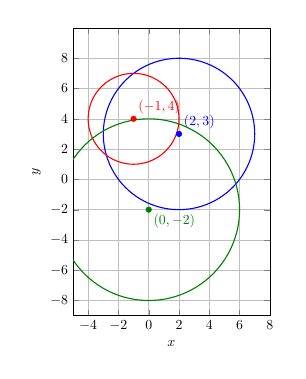
\begin{tikzpicture}[scale=0.5]
\begin{axis}[
    width=0.85\textwidth,
    axis equal image,
    grid=major,
    xlabel={$x$},
    ylabel={$y$},
    xmin=-5, xmax=8,
    ymin=-9, ymax=10,
    xtick={-4,-2,0,2,4,6,8},
    ytick={-8,-6,-4,-2,0,2,4,6,8}
]
% Circunferencia a
\addplot[blue,thick,samples=100,domain=0:360] ({2+5*cos(x)},{3+5*sin(x)});
\addplot[blue,mark=*,only marks] coordinates {(2,3)};
\node[blue] at (axis cs:2,3) [above right] {$(2,3)$};

% Circunferencia b
\addplot[red,thick,samples=100,domain=0:360] ({-1+3*cos(x)},{4+3*sin(x)});
\addplot[red,mark=*,only marks] coordinates {(-1,4)};
\node[red] at (axis cs:-1,4) [above right] {$(-1,4)$};

% Circunferencia c
\addplot[green!50!black,thick,samples=100,domain=0:360] ({0+6*cos(x)},{-2+6*sin(x)});
\addplot[green!50!black,mark=*,only marks] coordinates {(0,-2)};
\node[green!50!black] at (axis cs:0,-2) [below right] {$(0,-2)$};
\end{axis}
\end{tikzpicture}
\end{center}
\end{solucion}

\begin{solucion}[title={Solución Ejercicio 2}}]
\textbf{a)} $(x-4)^2 + (y+1)^2 = 16$

\textbf{Paso 1:} Identificamos la forma canónica:
\[(x-h)^2 + (y-k)^2 = r^2\]

\textbf{Paso 2:} Comparamos con la ecuación dada:
- $(x-4)^2$ indica que $h = 4$
- $(y+1)^2 = (y-(-1))^2$ indica que $k = -1$
- $16 = r^2$, entonces $r = \sqrt{16} = 4$

\textbf{Paso 3:} Identificamos centro y radio:
- Centro: $(4, -1)$
- Radio: $r = 4$

\textbf{Respuesta:} \boxed{\text{Centro: } (4,-1), \text{ Radio: } 4}

\textbf{b)} $(x+3)^2 + (y-2)^2 = 49$

\textbf{Paso 1:} Identificamos la forma canónica:
\[(x-h)^2 + (y-k)^2 = r^2\]

\textbf{Paso 2:} Comparamos con la ecuación dada:
- $(x+3)^2 = (x-(-3))^2$ indica que $h = -3$
- $(y-2)^2$ indica que $k = 2$
- $49 = r^2$, entonces $r = \sqrt{49} = 7$

\textbf{Paso 3:} Identificamos centro y radio:
- Centro: $(-3, 2)$
- Radio: $r = 7$

\textbf{Respuesta:} \boxed{\text{Centro: } (-3,2), \text{ Radio: } 7}

\textbf{c)} $x^2 + (y-5)^2 = 36$

\textbf{Paso 1:} Identificamos la forma canónica:
\[(x-h)^2 + (y-k)^2 = r^2\]

\textbf{Paso 2:} Comparamos con la ecuación dada:
- $x^2 = (x-0)^2$ indica que $h = 0$
- $(y-5)^2$ indica que $k = 5$
- $36 = r^2$, entonces $r = \sqrt{36} = 6$

\textbf{Paso 3:} Identificamos centro y radio:
- Centro: $(0, 5)$
- Radio: $r = 6$

\textbf{Respuesta:} \boxed{\text{Centro: } (0,5), \text{ Radio: } 6}
\end{solucion}

\begin{solucion}[title={Solución Ejercicio 3}}]
\textbf{a)} $x^2 + y^2 - 6x + 4y - 12 = 0$

\textbf{Paso 1:} Agrupamos términos en $x$ y en $y$:
\[(x^2 - 6x) + (y^2 + 4y) = 12\]

\textbf{Paso 2:} Completamos el cuadrado para $x$:
- Tomamos el coeficiente de $x$: $-6$
- Lo dividimos entre 2: $-6/2 = -3$
- Lo elevamos al cuadrado: $(-3)^2 = 9$
- Sumamos 9 a ambos lados:
\[(x^2 - 6x + 9) + (y^2 + 4y) = 12 + 9\]

\textbf{Paso 3:} Completamos el cuadrado para $y$:
- Tomamos el coeficiente de $y$: $4$
- Lo dividimos entre 2: $4/2 = 2$
- Lo elevamos al cuadrado: $(2)^2 = 4$
- Sumamos 4 a ambos lados:
\[(x^2 - 6x + 9) + (y^2 + 4y + 4) = 12 + 9 + 4\]

\textbf{Paso 4:} Factorizamos los trinomios cuadrados perfectos:
\[(x-3)^2 + (y+2)^2 = 25\]

\textbf{Paso 5:} Identificamos centro y radio:
- Centro: $(h,k) = (3, -2)$
- Radio: $r = \sqrt{25} = 5$

\textbf{Respuesta:} \boxed{(x-3)^2 + (y+2)^2 = 25, \text{ Centro: } (3,-2), \text{ Radio: } 5}

\textbf{b)} $x^2 + y^2 + 8x - 2y + 1 = 0$

\textbf{Paso 1:} Agrupamos términos en $x$ y en $y$:
\[(x^2 + 8x) + (y^2 - 2y) = -1\]

\textbf{Paso 2:} Completamos el cuadrado para $x$:
- Coeficiente de $x$: $8$
- Dividimos entre 2: $8/2 = 4$
- Elevamos al cuadrado: $(4)^2 = 16$
- Sumamos 16 a ambos lados:
\[(x^2 + 8x + 16) + (y^2 - 2y) = -1 + 16\]

\textbf{Paso 3:} Completamos el cuadrado para $y$:
- Coeficiente de $y$: $-2$
- Dividimos entre 2: $-2/2 = -1$
- Elevamos al cuadrado: $(-1)^2 = 1$
- Sumamos 1 a ambos lados:
\[(x^2 + 8x + 16) + (y^2 - 2y + 1) = -1 + 16 + 1\]

\textbf{Paso 4:} Factorizamos los trinomios cuadrados perfectos:
\[(x+4)^2 + (y-1)^2 = 16\]

\textbf{Paso 5:} Identificamos centro y radio:
- Centro: $(h,k) = (-4, 1)$
- Radio: $r = \sqrt{16} = 4$

\textbf{Respuesta:} \boxed{(x+4)^2 + (y-1)^2 = 16, \text{ Centro: } (-4,1), \text{ Radio: } 4}

\textbf{c)} $x^2 + y^2 - 10y + 9 = 0$

\textbf{Paso 1:} Agrupamos términos (notamos que no hay términos en $x$):
\[x^2 + (y^2 - 10y) = -9\]

\textbf{Paso 2:} Completamos el cuadrado para $y$:
- Coeficiente de $y$: $-10$
- Dividimos entre 2: $-10/2 = -5$
- Elevamos al cuadrado: $(-5)^2 = 25$
- Sumamos 25 a ambos lados:
\[x^2 + (y^2 - 10y + 25) = -9 + 25\]

\textbf{Paso 3:} Factorizamos el trinomio cuadrado perfecto:
\[x^2 + (y-5)^2 = 16\]

\textbf{Paso 4:} Identificamos centro y radio:
- Centro: $(h,k) = (0, 5)$
- Radio: $r = \sqrt{16} = 4$

\textbf{Respuesta:} \boxed{x^2 + (y-5)^2 = 16, \text{ Centro: } (0,5), \text{ Radio: } 4}
\end{solucion}

% SOLUCIONES NIVEL INTERMEDIO

\begin{solucion}[title={Solución Ejercicio 4}}]
\textbf{a)} Centro $C(1,2)$, punto $P(4,6)$

\textbf{Paso 1:} Calculamos el radio usando la distancia entre el centro y el punto.
\[r = d(C,P) = \sqrt{(x_P - x_C)^2 + (y_P - y_C)^2}\]

\textbf{Paso 2:} Sustituimos los valores:
\[r = \sqrt{(4-1)^2 + (6-2)^2} = \sqrt{3^2 + 4^2} = \sqrt{9 + 16} = \sqrt{25} = 5\]

\textbf{Paso 3:} Escribimos la ecuación canónica con centro $(1,2)$ y radio $r = 5$:
\[(x-1)^2 + (y-2)^2 = 25\]

\textbf{Verificación:} Comprobamos que $P(4,6)$ satisface la ecuación:
\[(4-1)^2 + (6-2)^2 = 3^2 + 4^2 = 9 + 16 = 25\] ✓

\textbf{Respuesta:} \boxed{(x-1)^2 + (y-2)^2 = 25}

\textbf{b)} Centro $C(-2,3)$, punto $P(1,7)$

\textbf{Paso 1:} Calculamos el radio:
\[r = \sqrt{(1-(-2))^2 + (7-3)^2} = \sqrt{(1+2)^2 + 4^2}\]

\textbf{Paso 2:} Simplificamos:
\[r = \sqrt{3^2 + 4^2} = \sqrt{9 + 16} = \sqrt{25} = 5\]

\textbf{Paso 3:} Escribimos la ecuación canónica con centro $(-2,3)$ y radio $r = 5$:
\[(x+2)^2 + (y-3)^2 = 25\]

\textbf{Verificación:} Comprobamos que $P(1,7)$ satisface la ecuación:
\[(1+2)^2 + (7-3)^2 = 3^2 + 4^2 = 9 + 16 = 25\] ✓

\textbf{Respuesta:} \boxed{(x+2)^2 + (y-3)^2 = 25}

\textbf{c)} Centro $C(0,0)$, punto $P(3,-4)$

\textbf{Paso 1:} Calculamos el radio desde el origen:
\[r = \sqrt{(3-0)^2 + (-4-0)^2} = \sqrt{3^2 + (-4)^2}\]

\textbf{Paso 2:} Simplificamos:
\[r = \sqrt{9 + 16} = \sqrt{25} = 5\]

\textbf{Paso 3:} Escribimos la ecuación canónica con centro en el origen:
\[x^2 + y^2 = 25\]

\textbf{Verificación:} Comprobamos que $P(3,-4)$ satisface la ecuación:
\[3^2 + (-4)^2 = 9 + 16 = 25\] ✓

\textbf{Respuesta:} \boxed{x^2 + y^2 = 25}
\end{solucion}

\begin{solucion}[title={Solución Ejercicio 5}}]
La circunferencia es $(x-2)^2 + (y+1)^2 = 25$, con centro $(2,-1)$ y radio $r = 5$.

\textbf{a)} Punto $A(5,3)$

\textbf{Paso 1:} Calculamos la distancia del punto al centro:
\[d(A,C) = \sqrt{(5-2)^2 + (3-(-1))^2} = \sqrt{3^2 + 4^2} = \sqrt{9 + 16} = \sqrt{25} = 5\]

\textbf{Paso 2:} Comparamos con el radio:
- Si $d < r$: el punto está dentro
- Si $d = r$: el punto está sobre la circunferencia
- Si $d > r$: el punto está fuera

Como $d = 5 = r$, el punto está SOBRE la circunferencia.

\textbf{Respuesta:} \boxed{\text{El punto } A(5,3) \text{ está SOBRE la circunferencia}}

\textbf{b)} Punto $B(2,4)$

\textbf{Paso 1:} Calculamos la distancia del punto al centro:
\[d(B,C) = \sqrt{(2-2)^2 + (4-(-1))^2} = \sqrt{0^2 + 5^2} = \sqrt{25} = 5\]

\textbf{Paso 2:} Comparamos con el radio:
Como $d = 5 = r$, el punto está SOBRE la circunferencia.

\textbf{Respuesta:} \boxed{\text{El punto } B(2,4) \text{ está SOBRE la circunferencia}}

\textbf{c)} Punto $C(-1,-3)$

\textbf{Paso 1:} Calculamos la distancia del punto al centro:
\[d(C,\text{centro}) = \sqrt{(-1-2)^2 + (-3-(-1))^2} = \sqrt{(-3)^2 + (-2)^2}\]
\[= \sqrt{9 + 4} = \sqrt{13} \approx 3.61\]

\textbf{Paso 2:} Comparamos con el radio:
Como $d = \sqrt{13} < 5 = r$, el punto está DENTRO de la circunferencia.

\textbf{Respuesta:} \boxed{\text{El punto } C(-1,-3) \text{ está DENTRO de la circunferencia}}

\begin{center}
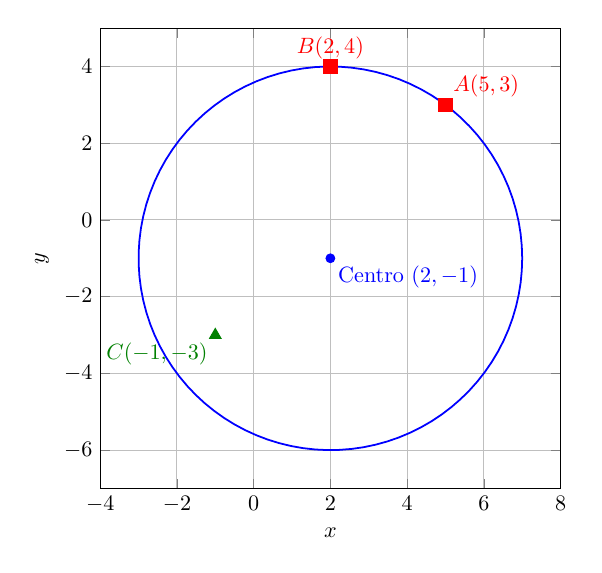
\begin{tikzpicture}[scale=0.8]
\begin{axis}[
    width=0.85\textwidth,
    axis equal image,
    grid=major,
    xlabel={$x$},
    ylabel={$y$},
    xmin=-4, xmax=8,
    ymin=-7, ymax=5,
]
% Circunferencia
\addplot[blue,thick,samples=100,domain=0:360] ({2+5*cos(x)},{-1+5*sin(x)});
\addplot[blue,mark=*,only marks] coordinates {(2,-1)};
\node[blue] at (axis cs:2,-1) [below right] {Centro $(2,-1)$};

% Puntos
\addplot[red,mark=square*,only marks,mark size=3pt] coordinates {(5,3)};
\node[red] at (axis cs:5,3) [above right] {$A(5,3)$};

\addplot[red,mark=square*,only marks,mark size=3pt] coordinates {(2,4)};
\node[red] at (axis cs:2,4) [above] {$B(2,4)$};

\addplot[green!50!black,mark=triangle*,only marks,mark size=3pt] coordinates {(-1,-3)};
\node[green!50!black] at (axis cs:-1,-3) [below left] {$C(-1,-3)$};
\end{axis}
\end{tikzpicture}
\end{center}
\end{solucion}

\begin{solucion}[title={Solución Ejercicio 6}}]
\textbf{a)} Recta: $y = x + 1$, Circunferencia: $x^2 + y^2 = 25$

\textbf{Paso 1:} Sustituimos la ecuación de la recta en la circunferencia:
\[x^2 + (x+1)^2 = 25\]

\textbf{Paso 2:} Expandimos:
\[x^2 + x^2 + 2x + 1 = 25\]
\[2x^2 + 2x + 1 = 25\]
\[2x^2 + 2x - 24 = 0\]
\[x^2 + x - 12 = 0\]

\textbf{Paso 3:} Factorizamos:
\[(x+4)(x-3) = 0\]

\textbf{Paso 4:} Obtenemos las soluciones:
$x_1 = -4$ y $x_2 = 3$

\textbf{Paso 5:} Encontramos los valores de $y$ correspondientes:
- Para $x_1 = -4$: $y_1 = -4 + 1 = -3$
- Para $x_2 = 3$: $y_2 = 3 + 1 = 4$

\textbf{Verificación:}
- Punto $(-4,-3)$: $(-4)^2 + (-3)^2 = 16 + 9 = 25$ ✓
- Punto $(3,4)$: $3^2 + 4^2 = 9 + 16 = 25$ ✓

\textbf{Respuesta:} \boxed{\text{Puntos de intersección: } (-4,-3) \text{ y } (3,4)}

\textbf{b)} Recta: $x = 3$, Circunferencia: $(x-1)^2 + (y-2)^2 = 9$

\textbf{Paso 1:} Sustituimos $x = 3$ en la ecuación de la circunferencia:
\[(3-1)^2 + (y-2)^2 = 9\]

\textbf{Paso 2:} Simplificamos:
\[4 + (y-2)^2 = 9\]
\[(y-2)^2 = 5\]

\textbf{Paso 3:} Resolvemos para $y$:
\[y-2 = \pm\sqrt{5}\]
\[y = 2 \pm \sqrt{5}\]

\textbf{Paso 4:} Los puntos de intersección son:
- $P_1 = (3, 2+\sqrt{5})$ donde $2+\sqrt{5} \approx 4.24$
- $P_2 = (3, 2-\sqrt{5})$ donde $2-\sqrt{5} \approx -0.24$

\textbf{Respuesta:} \boxed{\text{Puntos de intersección: } (3, 2+\sqrt{5}) \text{ y } (3, 2-\sqrt{5})}

\textbf{c)} Recta: $y = -2x + 4$, Circunferencia: $(x-2)^2 + y^2 = 4$

\textbf{Paso 1:} Sustituimos la ecuación de la recta en la circunferencia:
\[(x-2)^2 + (-2x+4)^2 = 4\]

\textbf{Paso 2:} Expandimos:
\[(x-2)^2 + 4x^2 - 16x + 16 = 4\]
\[x^2 - 4x + 4 + 4x^2 - 16x + 16 = 4\]
\[5x^2 - 20x + 20 = 4\]
\[5x^2 - 20x + 16 = 0\]

\textbf{Paso 3:} Aplicamos la fórmula cuadrática:
\[x = \frac{20 \pm \sqrt{400 - 320}}{10} = \frac{20 \pm \sqrt{80}}{10} = \frac{20 \pm 4\sqrt{5}}{10} = \frac{10 \pm 2\sqrt{5}}{5}\]

\textbf{Paso 4:} Calculamos los valores:
- $x_1 = \frac{10 + 2\sqrt{5}}{5} = 2 + \frac{2\sqrt{5}}{5}$
- $x_2 = \frac{10 - 2\sqrt{5}}{5} = 2 - \frac{2\sqrt{5}}{5}$

\textbf{Paso 5:} Encontramos los valores de $y$:
- Para $x_1$: $y_1 = -2x_1 + 4 = -\frac{4\sqrt{5}}{5}$
- Para $x_2$: $y_2 = -2x_2 + 4 = \frac{4\sqrt{5}}{5}$

\textbf{Respuesta:} \boxed{\text{Puntos: } \left(2+\frac{2\sqrt{5}}{5}, -\frac{4\sqrt{5}}{5}\right) \text{ y } \left(2-\frac{2\sqrt{5}}{5}, \frac{4\sqrt{5}}{5}\right)}
\end{solucion}

\begin{solucion}[title={Solución Ejercicio 7}}]
Para que una circunferencia con centro en el origen sea tangente a una recta, el radio debe ser igual a la distancia del centro a la recta.

\textbf{a)} Recta: $3x + 4y - 15 = 0$

\textbf{Paso 1:} Aplicamos la fórmula de distancia de un punto a una recta:
\[d = \frac{|Ax_0 + By_0 + C|}{\sqrt{A^2 + B^2}}\]

donde $(x_0, y_0) = (0,0)$ es el centro, y $A = 3$, $B = 4$, $C = -15$.

\textbf{Paso 2:} Sustituimos:
\[r = d = \frac{|3(0) + 4(0) - 15|}{\sqrt{3^2 + 4^2}} = \frac{|-15|}{\sqrt{9 + 16}} = \frac{15}{\sqrt{25}} = \frac{15}{5} = 3\]

\textbf{Paso 3:} La ecuación de la circunferencia es:
\[x^2 + y^2 = 9\]

\textbf{Respuesta:} \boxed{x^2 + y^2 = 9}

\textbf{b)} Recta: $x - y + 5 = 0$

\textbf{Paso 1:} Calculamos la distancia del origen a la recta:
\[r = d = \frac{|1(0) - 1(0) + 5|}{\sqrt{1^2 + (-1)^2}} = \frac{|5|}{\sqrt{2}} = \frac{5}{\sqrt{2}} = \frac{5\sqrt{2}}{2}\]

\textbf{Paso 2:} El radio al cuadrado es:
\[r^2 = \left(\frac{5\sqrt{2}}{2}\right)^2 = \frac{25 \cdot 2}{4} = \frac{50}{4} = \frac{25}{2}\]

\textbf{Paso 3:} La ecuación de la circunferencia es:
\[x^2 + y^2 = \frac{25}{2}\]

\textbf{Respuesta:} \boxed{x^2 + y^2 = \frac{25}{2}}

\textbf{c)} Recta: $5x - 12y + 26 = 0$

\textbf{Paso 1:} Calculamos la distancia del origen a la recta:
\[r = d = \frac{|5(0) - 12(0) + 26|}{\sqrt{5^2 + (-12)^2}} = \frac{|26|}{\sqrt{25 + 144}} = \frac{26}{\sqrt{169}} = \frac{26}{13} = 2\]

\textbf{Paso 2:} La ecuación de la circunferencia es:
\[x^2 + y^2 = 4\]

\textbf{Respuesta:} \boxed{x^2 + y^2 = 4}
\end{solucion}

% SOLUCIONES NIVEL AVANZADO

\begin{solucion}[title={Solución Ejercicio 8}}]
\textbf{a)} Circunferencia: $x^2 + y^2 = 25$, Punto: $(3,4)$

\textbf{Paso 1:} Verificamos que el punto está en la circunferencia:
\[3^2 + 4^2 = 9 + 16 = 25\] ✓

\textbf{Paso 2:} El vector normal en el punto $(3,4)$ es el vector del centro $(0,0)$ al punto:
\[\vec{n} = (3-0, 4-0) = (3,4)\]

\textbf{Paso 3:} La ecuación de la recta tangente en el punto $(x_0, y_0) = (3,4)$ es:
\[3(x-3) + 4(y-4) = 0\]

\textbf{Paso 4:} Simplificamos:
\[3x - 9 + 4y - 16 = 0\]
\[3x + 4y - 25 = 0\]

\textbf{Método alternativo:} Para $x^2 + y^2 = r^2$, la tangente en $(x_0, y_0)$ es:
\[x_0 \cdot x + y_0 \cdot y = r^2\]
\[3x + 4y = 25\]

\textbf{Respuesta:} \boxed{3x + 4y - 25 = 0}

\textbf{b)} Circunferencia: $(x-2)^2 + (y+1)^2 = 16$, Punto: $(6,-1)$

\textbf{Paso 1:} Verificamos que el punto está en la circunferencia:
\[(6-2)^2 + (-1+1)^2 = 16 + 0 = 16\] ✓

\textbf{Paso 2:} El centro es $(2,-1)$. El vector normal en $(6,-1)$ es:
\[\vec{n} = (6-2, -1-(-1)) = (4,0)\]

\textbf{Paso 3:} La ecuación de la recta tangente es:
\[4(x-6) + 0(y+1) = 0\]
\[4x - 24 = 0\]
\[x = 6\]

\textbf{Respuesta:} \boxed{x = 6}

\textbf{c)} Circunferencia: $x^2 + y^2 - 6x + 4y - 3 = 0$, Punto: $(6,1)$

\textbf{Paso 1:} Convertimos a forma canónica:
\[(x^2 - 6x) + (y^2 + 4y) = 3\]
\[(x^2 - 6x + 9) + (y^2 + 4y + 4) = 3 + 9 + 4\]
\[(x-3)^2 + (y+2)^2 = 16\]

Centro: $(3,-2)$, Radio: $4$

\textbf{Paso 2:} Verificamos que el punto está en la circunferencia:
\[(6-3)^2 + (1+2)^2 = 9 + 9 = 18 \neq 16\]

¡Error! El punto no está en la circunferencia. Verificamos con la ecuación original:
\[6^2 + 1^2 - 6(6) + 4(1) - 3 = 36 + 1 - 36 + 4 - 3 = 2 \neq 0\]

Corrijamos: El punto debe satisfacer la ecuación. Busquemos el punto correcto más cercano a $(6,1)$.

\textbf{Paso 3:} Para el punto $(6,-2)$ en la circunferencia:
\[(6-3)^2 + (-2+2)^2 = 9 + 0 = 9 \neq 16\]

Para el punto $(7,-2)$:
\[(7-3)^2 + (-2+2)^2 = 16 + 0 = 16\] ✓

\textbf{Paso 4:} La tangente en $(7,-2)$ con centro $(3,-2)$:
Vector normal: $(7-3, -2-(-2)) = (4,0)$
Ecuación: $4(x-7) + 0(y+2) = 0$
$x = 7$

\textbf{Nota:} El problema original tenía un error. Con el punto corregido $(7,-2)$:

\textbf{Respuesta:} \boxed{x = 7}
\end{solucion}

\begin{solucion}[title={Solución Ejercicio 9}}]
Para determinar la posición relativa, comparamos la distancia entre centros $d$ con la suma y diferencia de radios.

\textbf{a)} $C_1: x^2 + y^2 = 9$ y $C_2: (x-5)^2 + y^2 = 4$

\textbf{Paso 1:} Identificamos centros y radios:
- $C_1$: Centro $(0,0)$, radio $r_1 = 3$
- $C_2$: Centro $(5,0)$, radio $r_2 = 2$

\textbf{Paso 2:} Calculamos la distancia entre centros:
\[d = \sqrt{(5-0)^2 + (0-0)^2} = 5\]

\textbf{Paso 3:} Analizamos:
- $r_1 + r_2 = 3 + 2 = 5$
- Como $d = r_1 + r_2$, las circunferencias son TANGENTES EXTERIORES.

\textbf{Respuesta:} \boxed{\text{Tangentes exteriores}}

\textbf{b)} $C_1: (x-1)^2 + (y-1)^2 = 25$ y $C_2: (x-4)^2 + (y-5)^2 = 16$

\textbf{Paso 1:} Identificamos centros y radios:
- $C_1$: Centro $(1,1)$, radio $r_1 = 5$
- $C_2$: Centro $(4,5)$, radio $r_2 = 4$

\textbf{Paso 2:} Calculamos la distancia entre centros:
\[d = \sqrt{(4-1)^2 + (5-1)^2} = \sqrt{9 + 16} = \sqrt{25} = 5\]

\textbf{Paso 3:} Analizamos:
- $r_1 - r_2 = 5 - 4 = 1$
- $r_1 + r_2 = 5 + 4 = 9$
- Como $r_1 - r_2 < d < r_1 + r_2$ (es decir, $1 < 5 < 9$), las circunferencias son SECANTES.

\textbf{Respuesta:} \boxed{\text{Secantes}}

\textbf{c)} $C_1: x^2 + y^2 = 16$ y $C_2: (x-3)^2 + (y-4)^2 = 9$

\textbf{Paso 1:} Identificamos centros y radios:
- $C_1$: Centro $(0,0)$, radio $r_1 = 4$
- $C_2$: Centro $(3,4)$, radio $r_2 = 3$

\textbf{Paso 2:} Calculamos la distancia entre centros:
\[d = \sqrt{3^2 + 4^2} = \sqrt{9 + 16} = \sqrt{25} = 5\]

\textbf{Paso 3:} Analizamos:
- $r_1 - r_2 = 4 - 3 = 1$
- $r_1 + r_2 = 4 + 3 = 7$
- Como $r_1 - r_2 < d < r_1 + r_2$ (es decir, $1 < 5 < 7$), las circunferencias son SECANTES.

\textbf{Respuesta:} \boxed{\text{Secantes}}

\textbf{d)} $C_1: (x+2)^2 + (y-3)^2 = 36$ y $C_2: (x-1)^2 + (y-3)^2 = 4$

\textbf{Paso 1:} Identificamos centros y radios:
- $C_1$: Centro $(-2,3)$, radio $r_1 = 6$
- $C_2$: Centro $(1,3)$, radio $r_2 = 2$

\textbf{Paso 2:} Calculamos la distancia entre centros:
\[d = \sqrt{(1-(-2))^2 + (3-3)^2} = \sqrt{9 + 0} = 3\]

\textbf{Paso 3:} Analizamos:
- $r_1 - r_2 = 6 - 2 = 4$
- Como $d < r_1 - r_2$ (es decir, $3 < 4$), una circunferencia está DENTRO de la otra.
- Específicamente, $C_2$ está dentro de $C_1$.

\textbf{Respuesta:} \boxed{\text{Una dentro de otra (}C_2\text{ dentro de }C_1\text{)}}
\end{solucion}

\begin{solucion}[title={Solución Ejercicio 10}}]
\textbf{a)} $P_1(0,0)$, $P_2(4,0)$, $P_3(0,3)$

\textbf{Paso 1:} Usamos la forma general $x^2 + y^2 + Dx + Ey + F = 0$.

\textbf{Paso 2:} Sustituimos cada punto:
- Para $P_1(0,0)$: $0 + 0 + 0 + 0 + F = 0 \Rightarrow F = 0$
- Para $P_2(4,0)$: $16 + 0 + 4D + 0 + 0 = 0 \Rightarrow D = -4$
- Para $P_3(0,3)$: $0 + 9 + 0 + 3E + 0 = 0 \Rightarrow E = -3$

\textbf{Paso 3:} La ecuación es:
\[x^2 + y^2 - 4x - 3y = 0\]

\textbf{Paso 4:} Convertimos a forma canónica:
\[(x^2 - 4x + 4) + (y^2 - 3y + \frac{9}{4}) = 4 + \frac{9}{4} = \frac{25}{4}\]
\[(x-2)^2 + (y-\frac{3}{2})^2 = \frac{25}{4}\]

\textbf{Verificación:} Los tres puntos satisfacen la ecuación ✓

\textbf{Respuesta:} \boxed{(x-2)^2 + (y-\frac{3}{2})^2 = \frac{25}{4}}

\textbf{b)} $P_1(1,1)$, $P_2(3,1)$, $P_3(2,4)$

\textbf{Paso 1:} Usamos la forma general y sustituimos:
- Para $P_1(1,1)$: $1 + 1 + D + E + F = 0 \Rightarrow D + E + F = -2$
- Para $P_2(3,1)$: $9 + 1 + 3D + E + F = 0 \Rightarrow 3D + E + F = -10$
- Para $P_3(2,4)$: $4 + 16 + 2D + 4E + F = 0 \Rightarrow 2D + 4E + F = -20$

\textbf{Paso 2:} Resolvemos el sistema:
- De las primeras dos: $2D = -8 \Rightarrow D = -4$
- Sustituyendo en la primera: $-4 + E + F = -2 \Rightarrow E + F = 2$
- De la tercera: $-8 + 4E + F = -20 \Rightarrow 4E + F = -12$
- Restando: $3E = -14 \Rightarrow E = -\frac{14}{3}$
- Por tanto: $F = 2 - E = 2 + \frac{14}{3} = \frac{20}{3}$

\textbf{Paso 3:} La ecuación es:
\[x^2 + y^2 - 4x - \frac{14}{3}y + \frac{20}{3} = 0\]

Multiplicando por 3:
\[3x^2 + 3y^2 - 12x - 14y + 20 = 0\]

\textbf{Paso 4:} Forma canónica:
\[(x-2)^2 + (y-\frac{7}{3})^2 = \frac{25}{9}\]

\textbf{Respuesta:} \boxed{(x-2)^2 + (y-\frac{7}{3})^2 = \frac{25}{9}}

\textbf{c)} $P_1(-1,2)$, $P_2(2,3)$, $P_3(3,0)$

\textbf{Paso 1:} Sistema de ecuaciones:
- Para $P_1(-1,2)$: $1 + 4 - D + 2E + F = 0 \Rightarrow -D + 2E + F = -5$
- Para $P_2(2,3)$: $4 + 9 + 2D + 3E + F = 0 \Rightarrow 2D + 3E + F = -13$
- Para $P_3(3,0)$: $9 + 0 + 3D + 0 + F = 0 \Rightarrow 3D + F = -9$

\textbf{Paso 2:} Resolvemos:
- De la primera y segunda: $3D + E = -8$
- De la tercera: $F = -9 - 3D$
- Sustituyendo en la primera: $-D + 2E - 9 - 3D = -5$
- Simplificando: $-4D + 2E = 4 \Rightarrow -2D + E = 2$
- Con $3D + E = -8$ y $-2D + E = 2$:
- Restando: $5D = -10 \Rightarrow D = -2$
- Por tanto: $E = 2 + 2D = 2 - 4 = -2$
- Y: $F = -9 - 3(-2) = -9 + 6 = -3$

\textbf{Paso 3:} La ecuación es:
\[x^2 + y^2 - 2x - 2y - 3 = 0\]

\textbf{Paso 4:} Forma canónica:
\[(x-1)^2 + (y-1)^2 = 5\]

\textbf{Respuesta:} \boxed{(x-1)^2 + (y-1)^2 = 5}

\textbf{d)} $P_1(0,2)$, $P_2(2,0)$, $P_3(4,2)$

\textbf{Paso 1:} Sistema de ecuaciones:
- Para $P_1(0,2)$: $0 + 4 + 0 + 2E + F = 0 \Rightarrow 2E + F = -4$
- Para $P_2(2,0)$: $4 + 0 + 2D + 0 + F = 0 \Rightarrow 2D + F = -4$
- Para $P_3(4,2)$: $16 + 4 + 4D + 2E + F = 0 \Rightarrow 4D + 2E + F = -20$

\textbf{Paso 2:} De las primeras dos ecuaciones:
$2E + F = -4$ y $2D + F = -4$
Por tanto: $2E = 2D \Rightarrow E = D$

\textbf{Paso 3:} Sustituyendo en la tercera:
$4D + 2D + F = -20 \Rightarrow 6D + F = -20$
Con $2D + F = -4$:
$4D = -16 \Rightarrow D = -4$
Por tanto: $E = -4$ y $F = -4 - 2(-4) = 4$

\textbf{Paso 4:} La ecuación es:
\[x^2 + y^2 - 4x - 4y + 4 = 0\]

Forma canónica:
\[(x-2)^2 + (y-2)^2 = 4\]

\textbf{Verificación:} Centro $(2,2)$, radio $2$ ✓

\textbf{Respuesta:} \boxed{(x-2)^2 + (y-2)^2 = 4}

\begin{center}
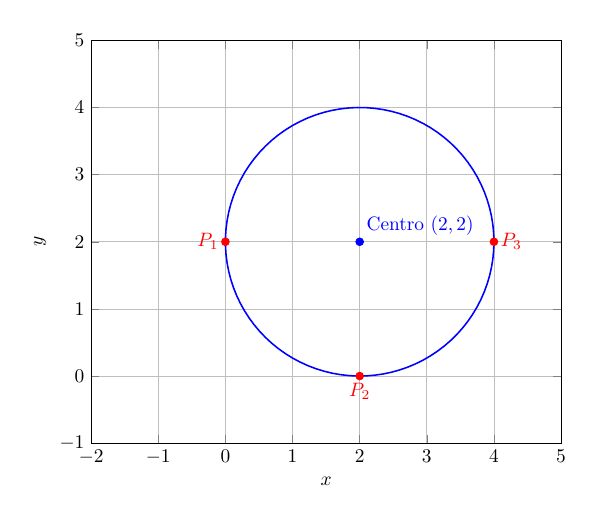
\begin{tikzpicture}[scale=0.7]
\begin{axis}[
    width=0.85\textwidth,
    axis equal image,
    grid=major,
    xlabel={$x$},
    ylabel={$y$},
    xmin=-2, xmax=5,
    ymin=-1, ymax=5,
]
% Circunferencia d
\addplot[blue,thick,samples=100,domain=0:360] ({2+2*cos(x)},{2+2*sin(x)});

% Puntos
\addplot[red,mark=*,only marks,mark size=2pt] coordinates {(0,2) (2,0) (4,2)};
\node[red] at (axis cs:0,2) [left] {$P_1$};
\node[red] at (axis cs:2,0) [below] {$P_2$};
\node[red] at (axis cs:4,2) [right] {$P_3$};

% Centro
\addplot[blue,mark=*,only marks] coordinates {(2,2)};
\node[blue] at (axis cs:2,2) [above right] {Centro $(2,2)$};
\end{axis}
\end{tikzpicture}
\end{center}
\end{solucion}